\documentclass[../Main.tex]{subfiles}

\begin{document}

\section{Visualización}
Con el objetivo de obtener una impresión de los datos, se procedió a graficar estos en bruto y buscar correlaciones entre los datos. 
\newline \par
Los sets del problema tienen los siguientes datos:
SAAF: Aspectos solares
\begin{center}
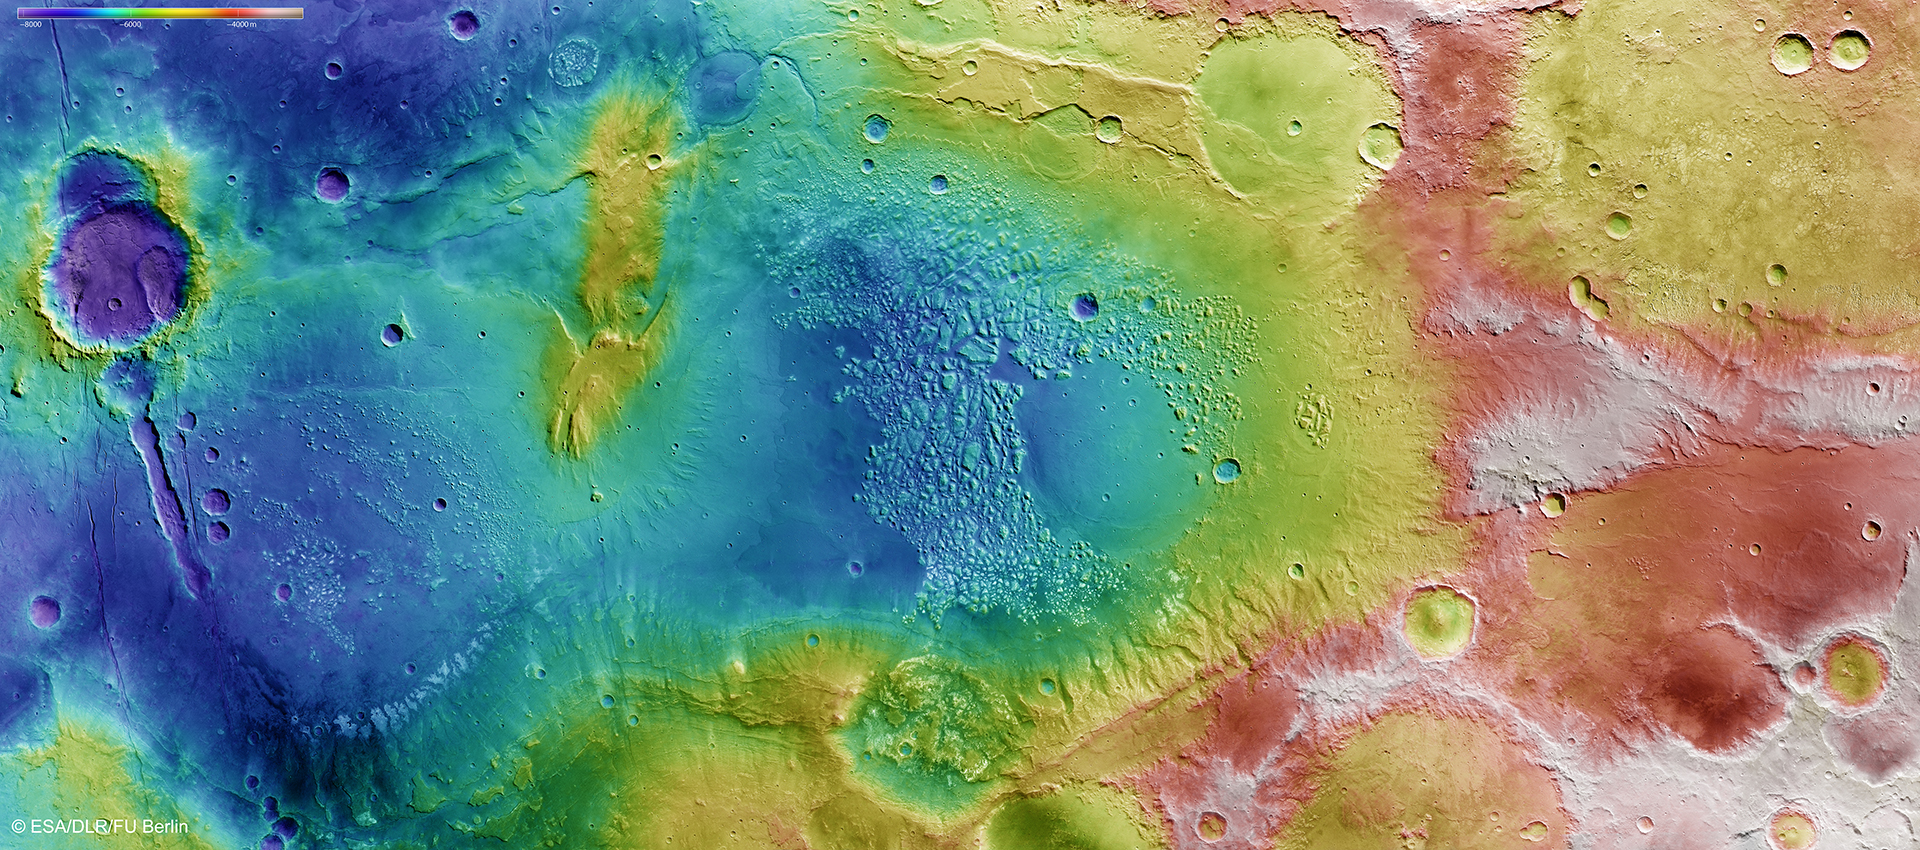
\includegraphics[width=\linewidth, trim={0 10cm 0 0}, clip]{Assets/Ancient_Atlantis.jpg}
\\Figura 1. Imágen con cotas del valle \textit{Ancient Atlantis}
\end{center}
DMOP: Detalles de la planificación de operación
\begin{center}
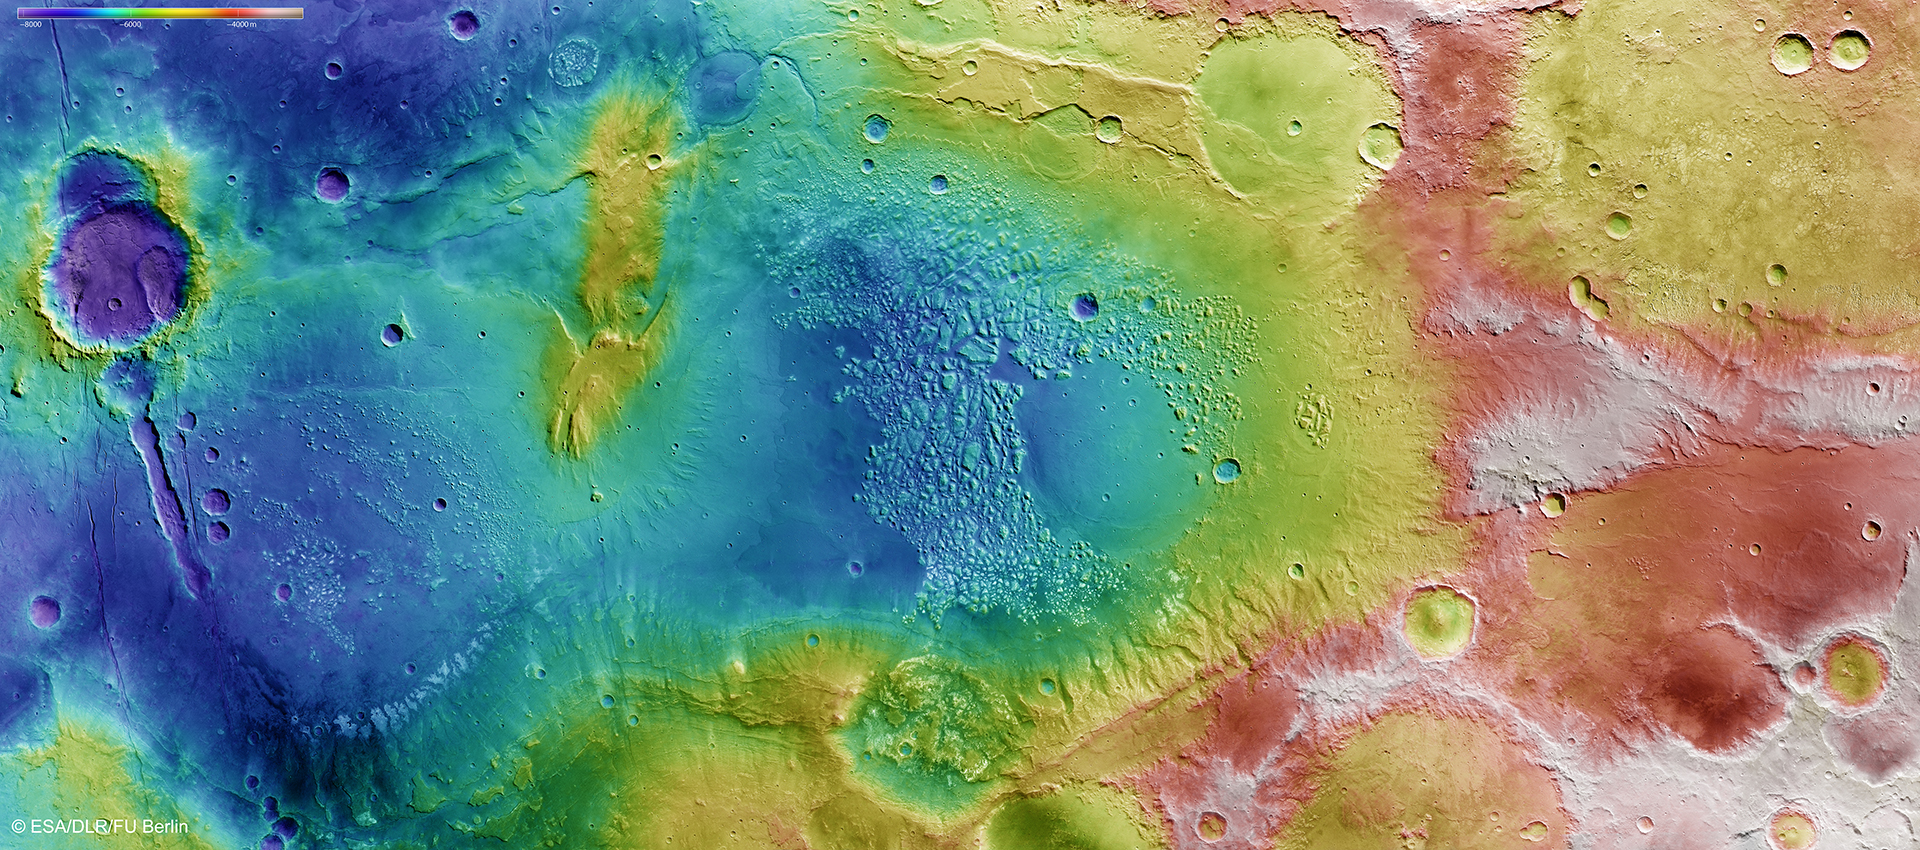
\includegraphics[width=\linewidth, trim={0 10cm 0 0}, clip]{Assets/Ancient_Atlantis.jpg}
\\Figura 1. Imágen con cotas del valle \textit{Ancient Atlantis}
\end{center}
FTL: Eventos de la trayectoria de la nave
\begin{center}
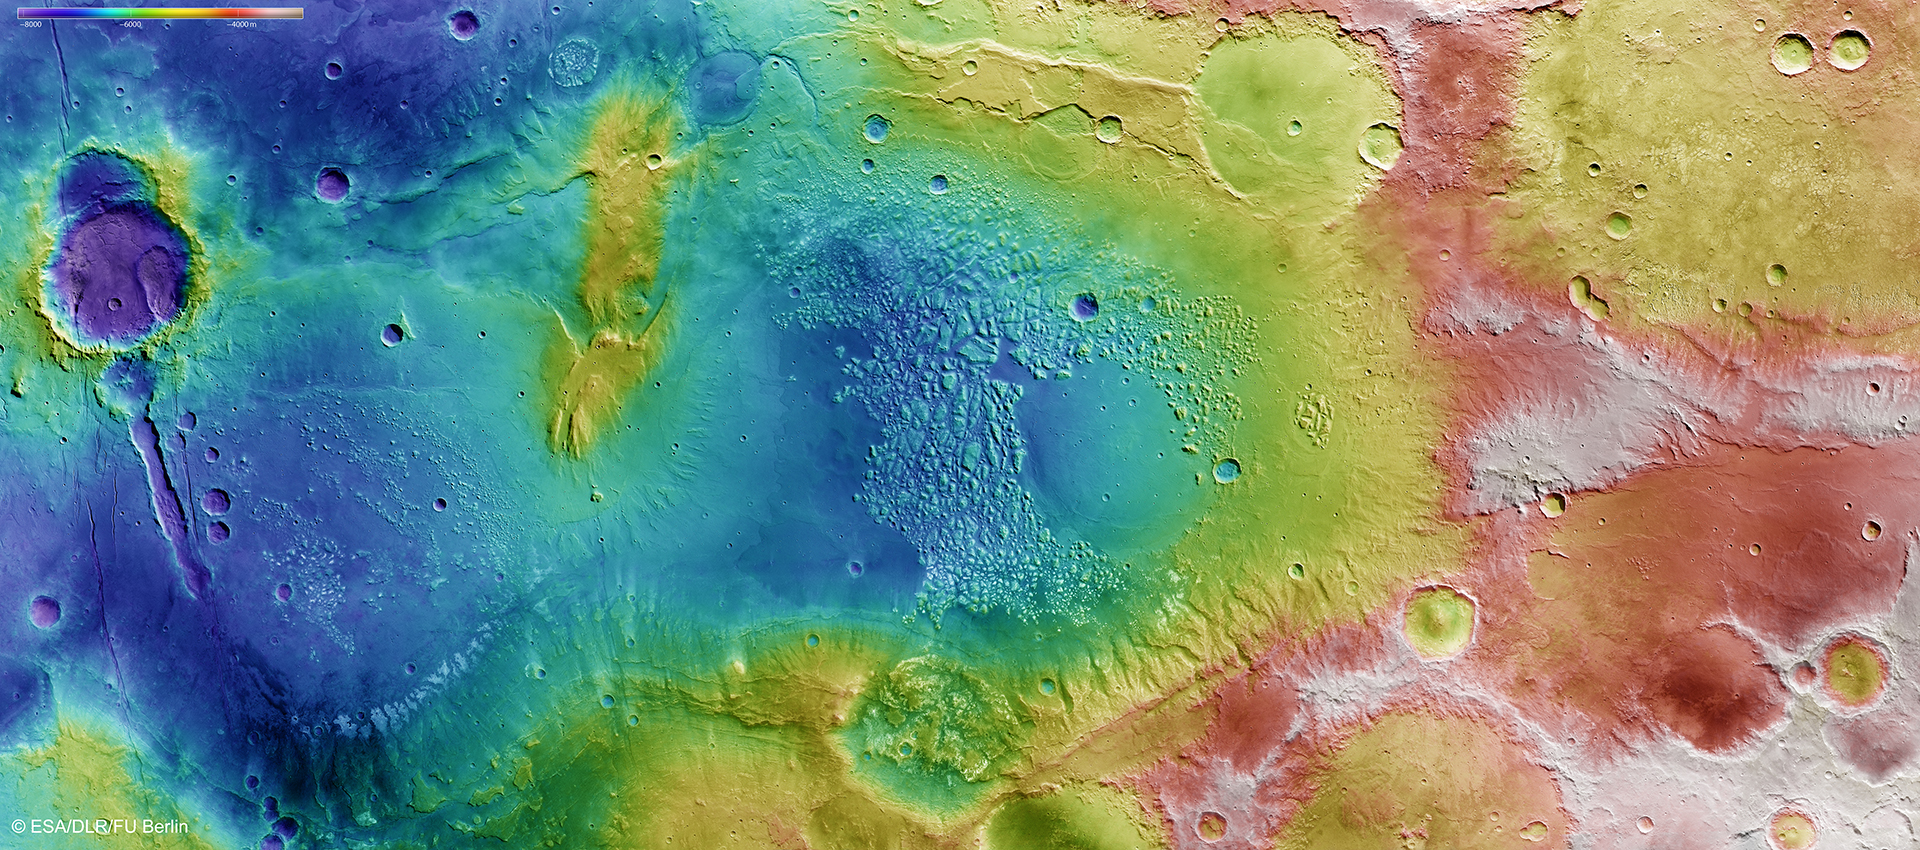
\includegraphics[width=\linewidth, trim={0 10cm 0 0}, clip]{Assets/Ancient_Atlantis.jpg}
\\Figura 1. Imágen con cotas del valle \textit{Ancient Atlantis}
\end{center}
EVTF: Otros eventos
\begin{center}
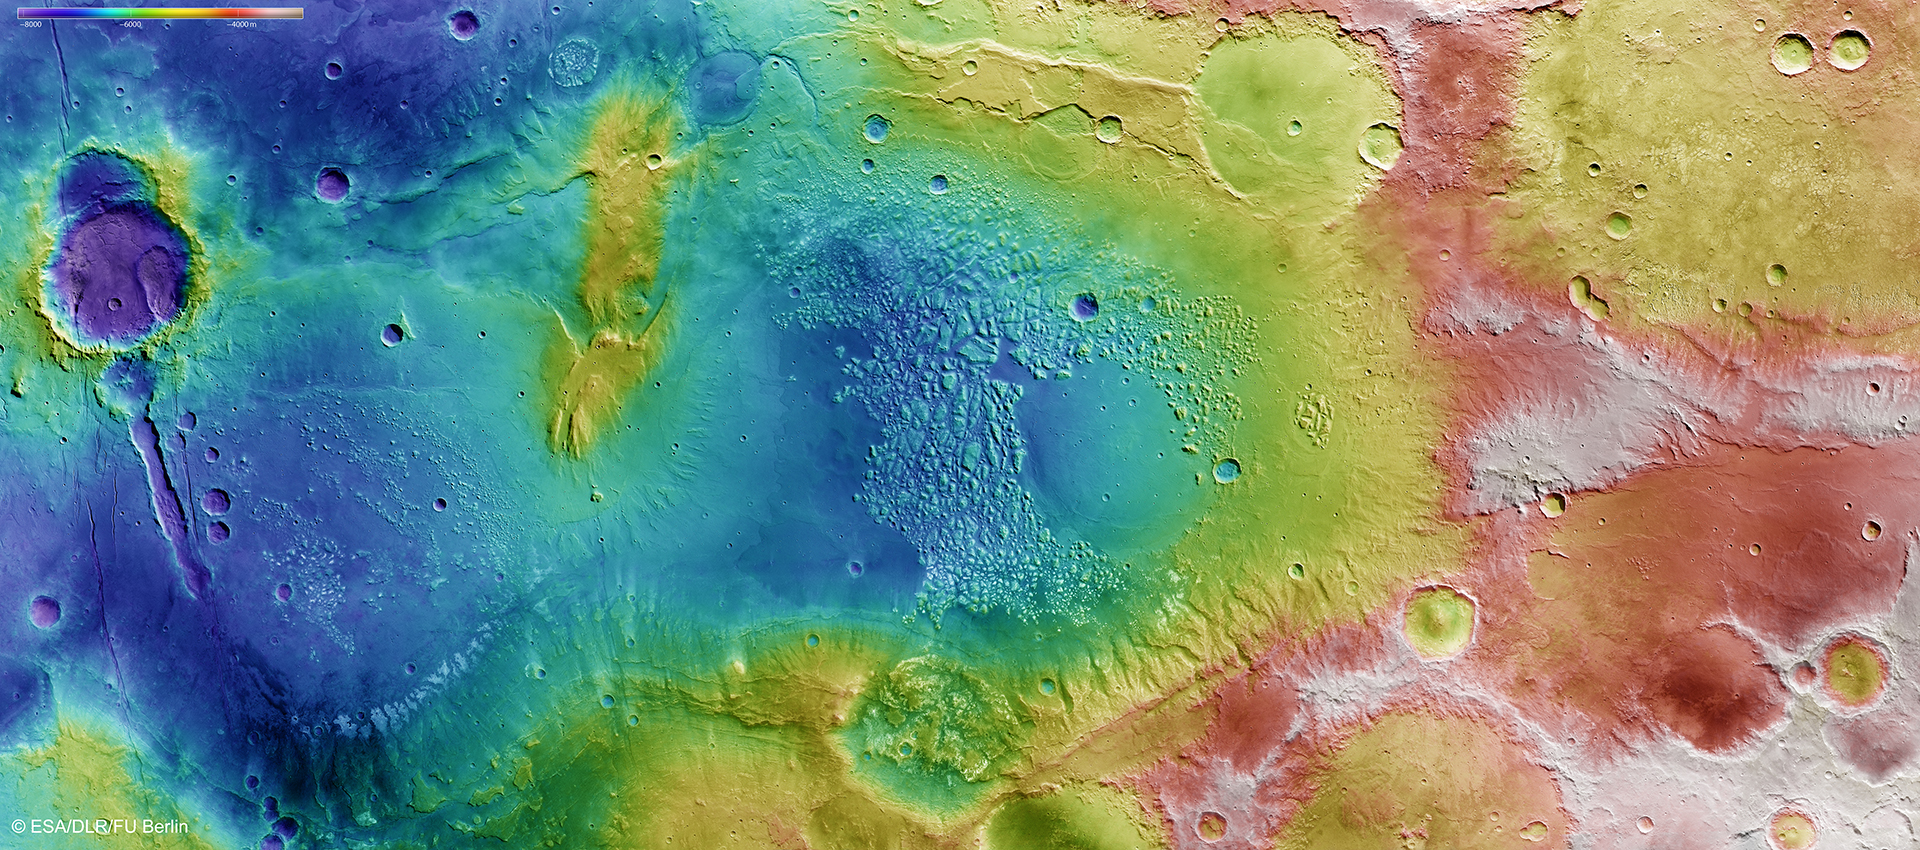
\includegraphics[width=\linewidth, trim={0 10cm 0 0}, clip]{Assets/Ancient_Atlantis.jpg}
\\Figura 1. Imágen con cotas del valle \textit{Ancient Atlantis}
\end{center}
LTDATA: Información de periodos extendidos
\begin{center}
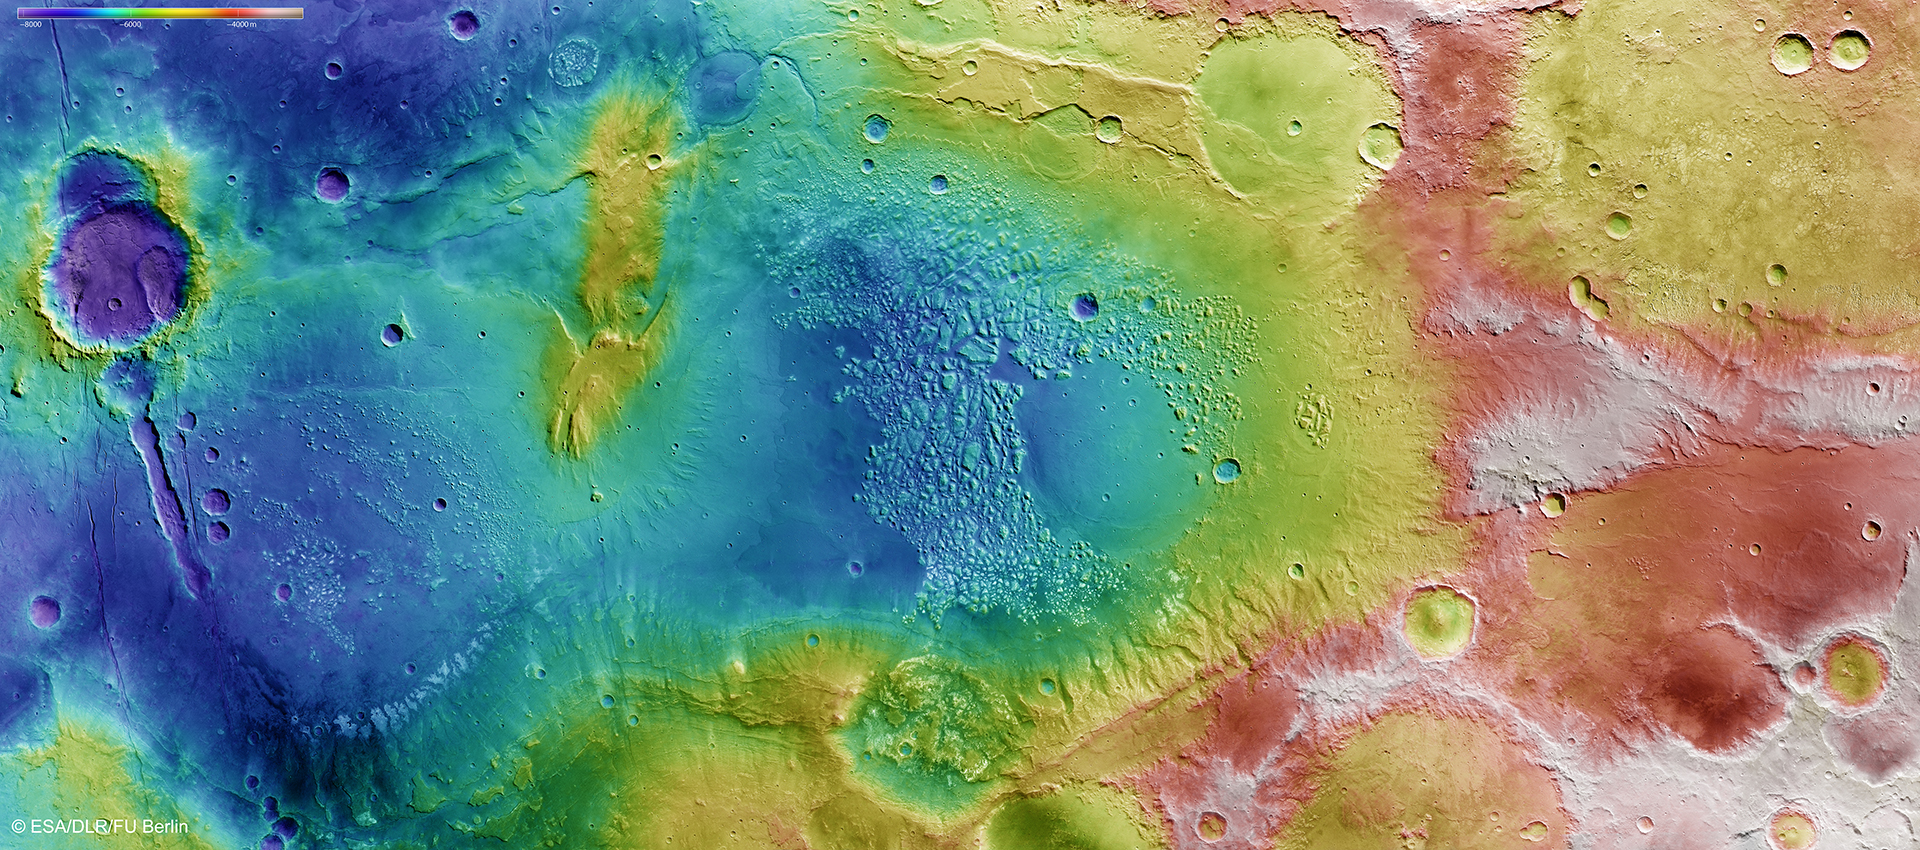
\includegraphics[width=\linewidth, trim={0 10cm 0 0}, clip]{Assets/Ancient_Atlantis.jpg}
\\Figura 1. Imágen con cotas del valle \textit{Ancient Atlantis}
\end{center}
POWER: Consumo energético
\begin{center}
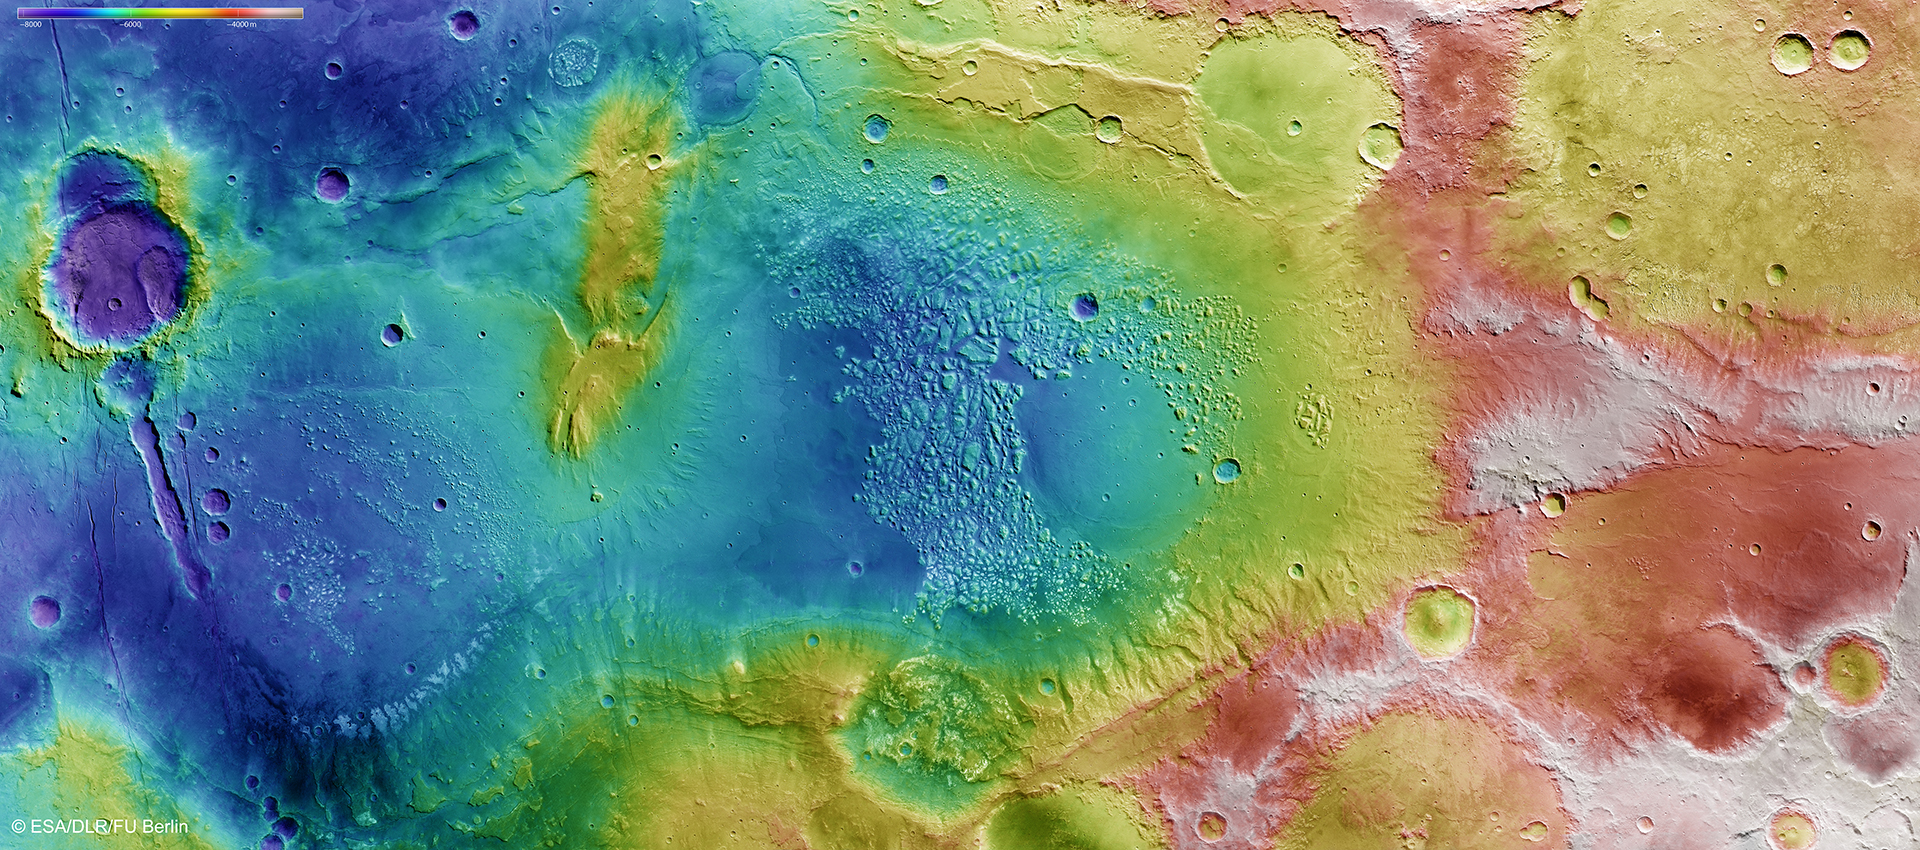
\includegraphics[width=\linewidth, trim={0 10cm 0 0}, clip]{Assets/Ancient_Atlantis.jpg}
\\Figura 1. Imágen con cotas del valle \textit{Ancient Atlantis}
\end{center}
\newline \par
Al graficar distintas variables por separado, se pueden obtener los siguientes gráficas:
%Graficas:
\newline \par
Al graficar los valores de potencia, los datos de incidencia solar y los datos de misión, se puede apreciar que existe una correlación entre los anteriores, por lo que se procedió a trabajar sobre estos datos en primera instancia. 
%Grafico de power1, saaf1 y ltdata1;
\newline \par
\end{document}